\documentclass[1p]{elsarticle_modified}
%\bibliographystyle{elsarticle-num}

%\usepackage[colorlinks]{hyperref}
%\usepackage{abbrmath_seonhwa} %\Abb, \Ascr, \Acal ,\Abf, \Afrak
\usepackage{amsfonts}
\usepackage{amssymb}
\usepackage{amsmath}
\usepackage{amsthm}
\usepackage{scalefnt}
\usepackage{amsbsy}
\usepackage{kotex}
\usepackage{caption}
\usepackage{subfig}
\usepackage{color}
\usepackage{graphicx}
\usepackage{xcolor} %% white, black, red, green, blue, cyan, magenta, yellow
\usepackage{float}
\usepackage{setspace}
\usepackage{hyperref}

\usepackage{tikz}
\usetikzlibrary{arrows}

\usepackage{multirow}
\usepackage{array} % fixed length table
\usepackage{hhline}

%%%%%%%%%%%%%%%%%%%%%
\makeatletter
\renewcommand*\env@matrix[1][\arraystretch]{%
	\edef\arraystretch{#1}%
	\hskip -\arraycolsep
	\let\@ifnextchar\new@ifnextchar
	\array{*\c@MaxMatrixCols c}}
\makeatother %https://tex.stackexchange.com/questions/14071/how-can-i-increase-the-line-spacing-in-a-matrix
%%%%%%%%%%%%%%%

\usepackage[normalem]{ulem}

\newcommand{\msout}[1]{\ifmmode\text{\sout{\ensuremath{#1}}}\else\sout{#1}\fi}
%SOURCE: \msout is \stkout macro in https://tex.stackexchange.com/questions/20609/strikeout-in-math-mode

\newcommand{\cancel}[1]{
	\ifmmode
	{\color{red}\msout{#1}}
	\else
	{\color{red}\sout{#1}}
	\fi
}

\newcommand{\add}[1]{
	{\color{blue}\uwave{#1}}
}

\newcommand{\replace}[2]{
	\ifmmode
	{\color{red}\msout{#1}}{\color{blue}\uwave{#2}}
	\else
	{\color{red}\sout{#1}}{\color{blue}\uwave{#2}}
	\fi
}

\newcommand{\Sol}{\mathcal{S}} %segment
\newcommand{\D}{D} %diagram
\newcommand{\A}{\mathcal{A}} %arc


%%%%%%%%%%%%%%%%%%%%%%%%%%%%%5 test

\def\sl{\operatorname{\textup{SL}}(2,\Cbb)}
\def\psl{\operatorname{\textup{PSL}}(2,\Cbb)}
\def\quan{\mkern 1mu \triangleright \mkern 1mu}

\theoremstyle{definition}
\newtheorem{thm}{Theorem}[section]
\newtheorem{prop}[thm]{Proposition}
\newtheorem{lem}[thm]{Lemma}
\newtheorem{ques}[thm]{Question}
\newtheorem{cor}[thm]{Corollary}
\newtheorem{defn}[thm]{Definition}
\newtheorem{exam}[thm]{Example}
\newtheorem{rmk}[thm]{Remark}
\newtheorem{alg}[thm]{Algorithm}

\newcommand{\I}{\sqrt{-1}}
\begin{document}

%\begin{frontmatter}
%
%\title{Boundary parabolic representations of knots up to 8 crossings}
%
%%% Group authors per affiliation:
%\author{Yunhi Cho} 
%\address{Department of Mathematics, University of Seoul, Seoul, Korea}
%\ead{yhcho@uos.ac.kr}
%
%
%\author{Seonhwa Kim} %\fnref{s_kim}}
%\address{Center for Geometry and Physics, Institute for Basic Science, Pohang, 37673, Korea}
%\ead{ryeona17@ibs.re.kr}
%
%\author{Hyuk Kim}
%\address{Department of Mathematical Sciences, Seoul National University, Seoul 08826, Korea}
%\ead{hyukkim@snu.ac.kr}
%
%\author{Seokbeom Yoon}
%\address{Department of Mathematical Sciences, Seoul National University, Seoul, 08826,  Korea}
%\ead{sbyoon15@snu.ac.kr}
%
%\begin{abstract}
%We find all boundary parabolic representation of knots up to 8 crossings.
%
%\end{abstract}
%\begin{keyword}
%    \MSC[2010] 57M25 
%\end{keyword}
%
%\end{frontmatter}

%\linenumbers
%\tableofcontents
%
\newcommand\colored[1]{\textcolor{white}{\rule[-0.35ex]{0.8em}{1.4ex}}\kern-0.8em\color{red} #1}%
%\newcommand\colored[1]{\textcolor{white}{ #1}\kern-2.17ex	\textcolor{white}{ #1}\kern-1.81ex	\textcolor{white}{ #1}\kern-2.15ex\color{red}#1	}

{\Large $\underline{12n_{0533}~(K12n_{0533})}$}

\setlength{\tabcolsep}{10pt}
\renewcommand{\arraystretch}{1.6}
\vspace{1cm}\begin{tabular}{m{100pt}>{\centering\arraybackslash}m{274pt}}
\multirow{5}{120pt}{
	\centering
	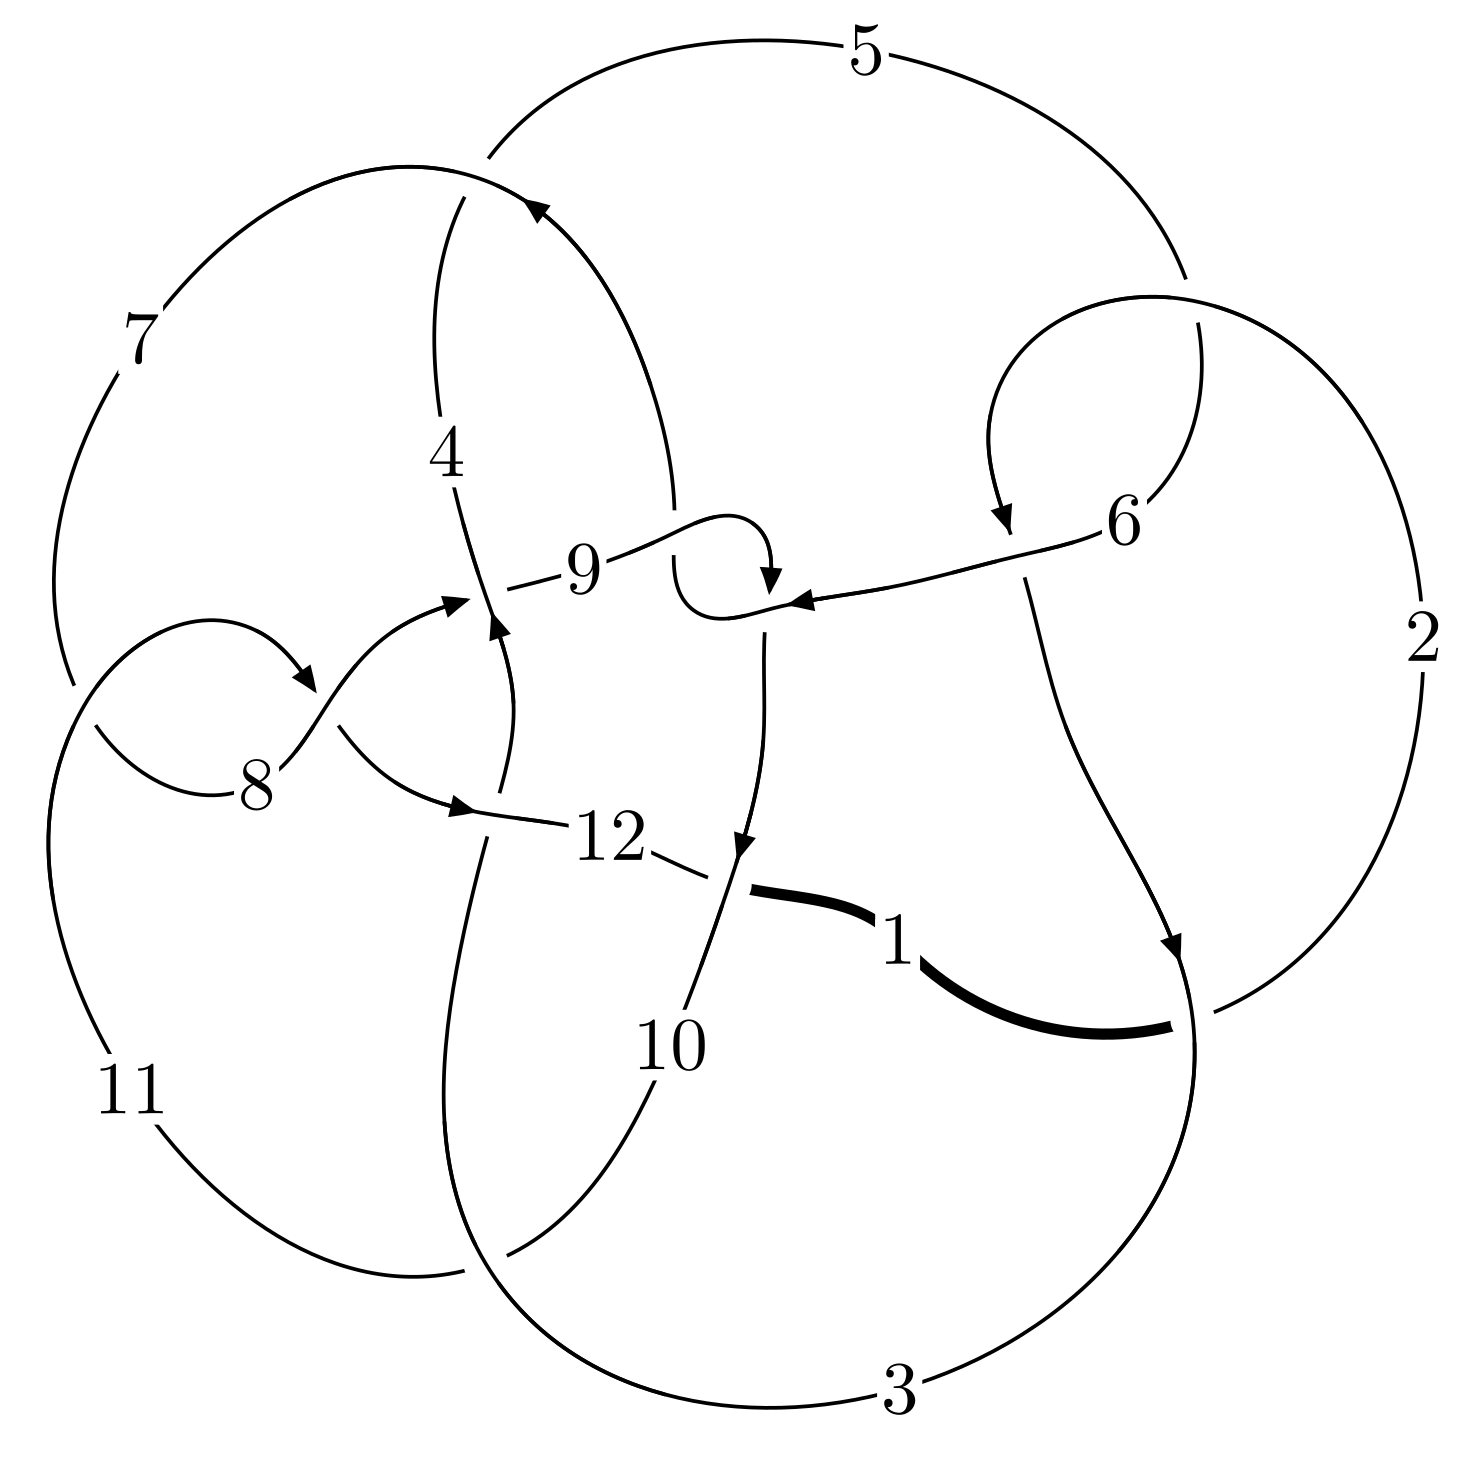
\includegraphics[width=112pt]{../../../GIT/diagram.site/Diagrams/png/2622_12n_0533.png}\\
\ \ \ A knot diagram\footnotemark}&
\allowdisplaybreaks
\textbf{Linearized knot diagam} \\
\cline{2-2}
 &
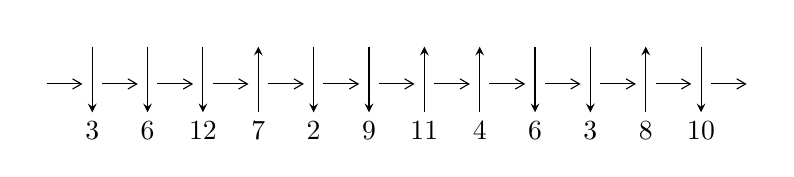
\begin{tikzpicture}[x=20pt, y=17pt]
	% nodes
	\node (C0) at (0, 0) {};
	\node (C1) at (1, 0) {};
	\node (C1U) at (1, +1) {};
	\node (C1D) at (1, -1) {3};

	\node (C2) at (2, 0) {};
	\node (C2U) at (2, +1) {};
	\node (C2D) at (2, -1) {6};

	\node (C3) at (3, 0) {};
	\node (C3U) at (3, +1) {};
	\node (C3D) at (3, -1) {12};

	\node (C4) at (4, 0) {};
	\node (C4U) at (4, +1) {};
	\node (C4D) at (4, -1) {7};

	\node (C5) at (5, 0) {};
	\node (C5U) at (5, +1) {};
	\node (C5D) at (5, -1) {2};

	\node (C6) at (6, 0) {};
	\node (C6U) at (6, +1) {};
	\node (C6D) at (6, -1) {9};

	\node (C7) at (7, 0) {};
	\node (C7U) at (7, +1) {};
	\node (C7D) at (7, -1) {11};

	\node (C8) at (8, 0) {};
	\node (C8U) at (8, +1) {};
	\node (C8D) at (8, -1) {4};

	\node (C9) at (9, 0) {};
	\node (C9U) at (9, +1) {};
	\node (C9D) at (9, -1) {6};

	\node (C10) at (10, 0) {};
	\node (C10U) at (10, +1) {};
	\node (C10D) at (10, -1) {3};

	\node (C11) at (11, 0) {};
	\node (C11U) at (11, +1) {};
	\node (C11D) at (11, -1) {8};

	\node (C12) at (12, 0) {};
	\node (C12U) at (12, +1) {};
	\node (C12D) at (12, -1) {10};
	\node (C13) at (13, 0) {};

	% arrows
	\draw[->,>={angle 60}]
	(C0) edge (C1) (C1) edge (C2) (C2) edge (C3) (C3) edge (C4) (C4) edge (C5) (C5) edge (C6) (C6) edge (C7) (C7) edge (C8) (C8) edge (C9) (C9) edge (C10) (C10) edge (C11) (C11) edge (C12) (C12) edge (C13) ;	\draw[->,>=stealth]
	(C1U) edge (C1D) (C2U) edge (C2D) (C3U) edge (C3D) (C4D) edge (C4U) (C5U) edge (C5D) (C6U) edge (C6D) (C7D) edge (C7U) (C8D) edge (C8U) (C9U) edge (C9D) (C10U) edge (C10D) (C11D) edge (C11U) (C12U) edge (C12D) ;
	\end{tikzpicture} \\
\hhline{~~} \\& 
\textbf{Solving Sequence} \\ \cline{2-2} 
 &
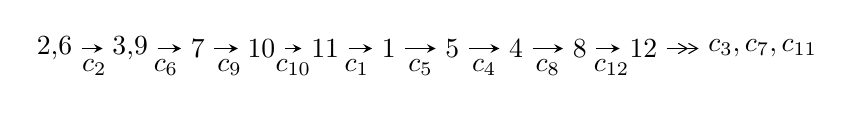
\begin{tikzpicture}[x=23pt, y=7pt]
	% node
	\node (A0) at (-1/8, 0) {2,6};
	\node (A1) at (17/16, 0) {3,9};
	\node (A2) at (17/8, 0) {7};
	\node (A3) at (25/8, 0) {10};
	\node (A4) at (33/8, 0) {11};
	\node (A5) at (41/8, 0) {1};
	\node (A6) at (49/8, 0) {5};
	\node (A7) at (57/8, 0) {4};
	\node (A8) at (65/8, 0) {8};
	\node (A9) at (73/8, 0) {12};
	\node (C1) at (1/2, -1) {$c_{2}$};
	\node (C2) at (13/8, -1) {$c_{6}$};
	\node (C3) at (21/8, -1) {$c_{9}$};
	\node (C4) at (29/8, -1) {$c_{10}$};
	\node (C5) at (37/8, -1) {$c_{1}$};
	\node (C6) at (45/8, -1) {$c_{5}$};
	\node (C7) at (53/8, -1) {$c_{4}$};
	\node (C8) at (61/8, -1) {$c_{8}$};
	\node (C9) at (69/8, -1) {$c_{12}$};
	\node (A10) at (11, 0) {$c_{3},c_{7},c_{11}$};

	% edge
	\draw[->,>=stealth]	
	(A0) edge (A1) (A1) edge (A2) (A2) edge (A3) (A3) edge (A4) (A4) edge (A5) (A5) edge (A6) (A6) edge (A7) (A7) edge (A8) (A8) edge (A9) ;
	\draw[->>,>={angle 60}]	
	(A9) edge (A10);
\end{tikzpicture} \\ 

\end{tabular} \\

\footnotetext{
The image of knot diagram is generated by the software ``\textbf{Draw programme}" developed by Andrew Bartholomew(\url{http://www.layer8.co.uk/maths/draw/index.htm\#Running-draw}), where we modified some parts for our purpose(\url{https://github.com/CATsTAILs/LinksPainter}).
}\phantom \\ \newline 
\centering \textbf{Ideals for irreducible components\footnotemark of $X_{\text{par}}$} 
 
\begin{align*}
I^u_{1}&=\langle 
b- u,\;685852313 u^{18}-556454916 u^{17}+\cdots+653732120 a+7160013,\;u^{19}- u^{18}+\cdots- u-1\rangle \\
I^u_{2}&=\langle 
-5.47513\times10^{57} u^{27}-1.03765\times10^{58} u^{26}+\cdots+1.25931\times10^{60} b+3.43121\times10^{60},\\
\phantom{I^u_{2}}&\phantom{= \langle  }2.52837\times10^{60} u^{27}+8.41887\times10^{58} u^{26}+\cdots+3.70867\times10^{62} a-9.79223\times10^{62},\\
\phantom{I^u_{2}}&\phantom{= \langle  }2 u^{28}-31 u^{26}+\cdots-1810 u+589\rangle \\
I^u_{3}&=\langle 
b+u,\;2 u^8+8 u^7+6 u^6-13 u^5-23 u^4-10 u^3+3 u^2+a+3 u+1,\\
\phantom{I^u_{3}}&\phantom{= \langle  }u^9+4 u^8+3 u^7-7 u^6-13 u^5-5 u^4+5 u^3+4 u^2-1\rangle \\
I^u_{4}&=\langle 
b+1,\;3 a-4 u-2,\;2 u^2+4 u+3\rangle \\
I^u_{5}&=\langle 
b+1,\;a^2+2,\;u-1\rangle \\
I^u_{6}&=\langle 
2 b- a-2,\;a^2+2,\;u-1\rangle \\
I^u_{7}&=\langle 
b+1,\;a,\;u-1\rangle \\
\\
\end{align*}
\raggedright * 7 irreducible components of $\dim_{\mathbb{C}}=0$, with total 63 representations.\\
\footnotetext{All coefficients of polynomials are rational numbers. But the coefficients are sometimes approximated in decimal forms when there is not enough margin.}
\newpage
\renewcommand{\arraystretch}{1}
\centering \section*{I. $I^u_{1}= \langle b- u,\;6.86\times10^{8} u^{18}-5.56\times10^{8} u^{17}+\cdots+6.54\times10^{8} a+7.16\times10^{6},\;u^{19}- u^{18}+\cdots- u-1 \rangle$}
\flushleft \textbf{(i) Arc colorings}\\
\begin{tabular}{m{7pt} m{180pt} m{7pt} m{180pt} }
\flushright $a_{2}=$&$\begin{pmatrix}1\\0\end{pmatrix}$ \\
\flushright $a_{6}=$&$\begin{pmatrix}0\\u\end{pmatrix}$ \\
\flushright $a_{3}=$&$\begin{pmatrix}1\\u^2\end{pmatrix}$ \\
\flushright $a_{9}=$&$\begin{pmatrix}-1.04913 u^{18}+0.851197 u^{17}+\cdots+7.34496 u-0.0109525\\u\end{pmatrix}$ \\
\flushright $a_{7}=$&$\begin{pmatrix}0.158099 u^{18}+0.275222 u^{17}+\cdots-2.08930 u-3.03953\\-0.293094 u^{18}+0.271534 u^{17}+\cdots+2.24707 u+0.197936\end{pmatrix}$ \\
\flushright $a_{10}=$&$\begin{pmatrix}-1.04913 u^{18}+0.851197 u^{17}+\cdots+7.34496 u-0.0109525\\0.293094 u^{18}-0.271534 u^{17}+\cdots-0.247070 u-0.197936\end{pmatrix}$ \\
\flushright $a_{11}=$&$\begin{pmatrix}-1.04913 u^{18}+0.851197 u^{17}+\cdots+6.34496 u-0.0109525\\0.293094 u^{18}-0.271534 u^{17}+\cdots-0.247070 u-0.197936\end{pmatrix}$ \\
\flushright $a_{1}=$&$\begin{pmatrix}- u^2+1\\- u^4\end{pmatrix}$ \\
\flushright $a_{5}=$&$\begin{pmatrix}u\\u\end{pmatrix}$ \\
\flushright $a_{4}=$&$\begin{pmatrix}-0.0634274 u^{18}-0.299411 u^{17}+\cdots-0.158823 u+2.17783\\0.309916 u^{18}-0.197991 u^{17}+\cdots-0.689516 u-0.693690\end{pmatrix}$ \\
\flushright $a_{8}=$&$\begin{pmatrix}-0.489325 u^{18}+0.908085 u^{17}+\cdots+2.86952 u-2.02077\\0.146260 u^{18}-0.320706 u^{17}+\cdots+1.12146 u+0.224248\end{pmatrix}$ \\
\flushright $a_{12}=$&$\begin{pmatrix}0.652817 u^{18}-1.22239 u^{17}+\cdots-1.72619 u+2.50033\\-0.0560035 u^{18}+0.251833 u^{17}+\cdots-0.0119146 u-0.862668\end{pmatrix}$\\&\end{tabular}
\flushleft \textbf{(ii) Obstruction class $= -1$}\\~\\
\flushleft \textbf{(iii) Cusp Shapes $= -\frac{98599477}{81716515} u^{18}+\frac{19045887}{32686606} u^{17}+\cdots+\frac{1773159057}{163433030} u+\frac{96551023}{32686606}$}\\~\\
\newpage\renewcommand{\arraystretch}{1}
\flushleft \textbf{(iv) u-Polynomials at the component}\newline \\
\begin{tabular}{m{50pt}|m{274pt}}
Crossings & \hspace{64pt}u-Polynomials at each crossing \\
\hline $$\begin{aligned}c_{1}\end{aligned}$$&$\begin{aligned}
&u^{19}+29 u^{18}+\cdots-21 u+1
\end{aligned}$\\
\hline $$\begin{aligned}c_{2},c_{5},c_{10}\end{aligned}$$&$\begin{aligned}
&u^{19}+u^{18}+\cdots- u+1
\end{aligned}$\\
\hline $$\begin{aligned}c_{3}\end{aligned}$$&$\begin{aligned}
&u^{19}-12 u^{18}+\cdots-112 u+8
\end{aligned}$\\
\hline $$\begin{aligned}c_{4}\end{aligned}$$&$\begin{aligned}
&u^{19}+u^{18}+\cdots+38 u+19
\end{aligned}$\\
\hline $$\begin{aligned}c_{6},c_{9}\end{aligned}$$&$\begin{aligned}
&u^{19}-11 u^{18}+\cdots+192 u-16
\end{aligned}$\\
\hline $$\begin{aligned}c_{7},c_{8},c_{11}\end{aligned}$$&$\begin{aligned}
&u^{19}-6 u^{17}+\cdots+2 u+1
\end{aligned}$\\
\hline $$\begin{aligned}c_{12}\end{aligned}$$&$\begin{aligned}
&u^{19}-2 u^{18}+\cdots+640 u+206
\end{aligned}$\\
\hline
\end{tabular}\\~\\
\newpage\renewcommand{\arraystretch}{1}
\flushleft \textbf{(v) Riley Polynomials at the component}\newline \\
\begin{tabular}{m{50pt}|m{274pt}}
Crossings & \hspace{64pt}Riley Polynomials at each crossing \\
\hline $$\begin{aligned}c_{1}\end{aligned}$$&$\begin{aligned}
&y^{19}-89 y^{18}+\cdots+167 y-1
\end{aligned}$\\
\hline $$\begin{aligned}c_{2},c_{5},c_{10}\end{aligned}$$&$\begin{aligned}
&y^{19}-29 y^{18}+\cdots-21 y-1
\end{aligned}$\\
\hline $$\begin{aligned}c_{3}\end{aligned}$$&$\begin{aligned}
&y^{19}+4 y^{18}+\cdots+2272 y-64
\end{aligned}$\\
\hline $$\begin{aligned}c_{4}\end{aligned}$$&$\begin{aligned}
&y^{19}+17 y^{18}+\cdots+342 y-361
\end{aligned}$\\
\hline $$\begin{aligned}c_{6},c_{9}\end{aligned}$$&$\begin{aligned}
&y^{19}+9 y^{18}+\cdots+10112 y-256
\end{aligned}$\\
\hline $$\begin{aligned}c_{7},c_{8},c_{11}\end{aligned}$$&$\begin{aligned}
&y^{19}-12 y^{18}+\cdots+20 y-1
\end{aligned}$\\
\hline $$\begin{aligned}c_{12}\end{aligned}$$&$\begin{aligned}
&y^{19}-44 y^{18}+\cdots+39624 y-42436
\end{aligned}$\\
\hline
\end{tabular}\\~\\
\newpage\flushleft \textbf{(vi) Complex Volumes and Cusp Shapes}
$$\begin{array}{c|c|c}  
\text{Solutions to }I^u_{1}& \I (\text{vol} + \sqrt{-1}CS) & \text{Cusp shape}\\
 \hline 
\begin{aligned}
u &= \phantom{-}1.011380 + 0.313488 I \\
a &= \phantom{-}0.32432 + 1.42243 I \\
b &= \phantom{-}1.011380 + 0.313488 I\end{aligned}
 & \phantom{-}3.19066 + 0.85534 I & -5.53948 - 2.70144 I \\ \hline\begin{aligned}
u &= \phantom{-}1.011380 - 0.313488 I \\
a &= \phantom{-}0.32432 - 1.42243 I \\
b &= \phantom{-}1.011380 - 0.313488 I\end{aligned}
 & \phantom{-}3.19066 - 0.85534 I & -5.53948 + 2.70144 I \\ \hline\begin{aligned}
u &= -0.563817 + 0.542216 I \\
a &= -1.26815 + 1.02395 I \\
b &= -0.563817 + 0.542216 I\end{aligned}
 & \phantom{-}7.09944 + 1.17461 I & \phantom{-}4.73931 - 3.05170 I \\ \hline\begin{aligned}
u &= -0.563817 - 0.542216 I \\
a &= -1.26815 - 1.02395 I \\
b &= -0.563817 - 0.542216 I\end{aligned}
 & \phantom{-}7.09944 - 1.17461 I & \phantom{-}4.73931 + 3.05170 I \\ \hline\begin{aligned}
u &= \phantom{-}0.678408\phantom{ +0.000000I} \\
a &= \phantom{-}0.230292\phantom{ +0.000000I} \\
b &= \phantom{-}0.678408\phantom{ +0.000000I}\end{aligned}
 & -1.17152\phantom{ +0.000000I} & -9.47840\phantom{ +0.000000I} \\ \hline\begin{aligned}
u &= -0.102826 + 0.584964 I \\
a &= \phantom{-}1.67025 - 1.13096 I \\
b &= -0.102826 + 0.584964 I\end{aligned}
 & \phantom{-}4.80007 - 6.25425 I & \phantom{-}1.28229 + 2.73136 I \\ \hline\begin{aligned}
u &= -0.102826 - 0.584964 I \\
a &= \phantom{-}1.67025 + 1.13096 I \\
b &= -0.102826 - 0.584964 I\end{aligned}
 & \phantom{-}4.80007 + 6.25425 I & \phantom{-}1.28229 - 2.73136 I \\ \hline\begin{aligned}
u &= -0.263709 + 0.494501 I \\
a &= -0.994354 - 0.913393 I \\
b &= -0.263709 + 0.494501 I\end{aligned}
 & \phantom{-}2.36863 - 1.74565 I & -1.37224 + 0.88301 I \\ \hline\begin{aligned}
u &= -0.263709 - 0.494501 I \\
a &= -0.994354 + 0.913393 I \\
b &= -0.263709 - 0.494501 I\end{aligned}
 & \phantom{-}2.36863 + 1.74565 I & -1.37224 - 0.88301 I \\ \hline\begin{aligned}
u &= -0.006101 + 0.333119 I \\
a &= -2.12160 + 1.28521 I \\
b &= -0.006101 + 0.333119 I\end{aligned}
 & \phantom{-}0.09772 - 1.41403 I & \phantom{-}1.26259 + 3.76239 I\\
 \hline 
 \end{array}$$\newpage$$\begin{array}{c|c|c}  
\text{Solutions to }I^u_{1}& \I (\text{vol} + \sqrt{-1}CS) & \text{Cusp shape}\\
 \hline 
\begin{aligned}
u &= -0.006101 - 0.333119 I \\
a &= -2.12160 - 1.28521 I \\
b &= -0.006101 - 0.333119 I\end{aligned}
 & \phantom{-}0.09772 + 1.41403 I & \phantom{-}1.26259 - 3.76239 I \\ \hline\begin{aligned}
u &= -1.82852 + 0.27307 I \\
a &= -0.568825 + 0.667950 I \\
b &= -1.82852 + 0.27307 I\end{aligned}
 & -9.74488 + 5.38592 I & -1.90391 - 4.79888 I \\ \hline\begin{aligned}
u &= -1.82852 - 0.27307 I \\
a &= -0.568825 - 0.667950 I \\
b &= -1.82852 - 0.27307 I\end{aligned}
 & -9.74488 - 5.38592 I & -1.90391 + 4.79888 I \\ \hline\begin{aligned}
u &= \phantom{-}1.90401 + 0.14512 I \\
a &= \phantom{-}0.798373 + 0.448929 I \\
b &= \phantom{-}1.90401 + 0.14512 I\end{aligned}
 & -8.63257 + 5.48554 I & -4.82467 - 3.57754 I \\ \hline\begin{aligned}
u &= \phantom{-}1.90401 - 0.14512 I \\
a &= \phantom{-}0.798373 - 0.448929 I \\
b &= \phantom{-}1.90401 - 0.14512 I\end{aligned}
 & -8.63257 - 5.48554 I & -4.82467 + 3.57754 I \\ \hline\begin{aligned}
u &= -1.90239 + 0.21588 I \\
a &= -0.651528 + 0.330559 I \\
b &= -1.90239 + 0.21588 I\end{aligned}
 & -11.79520 + 2.21872 I & -6.42414 + 1.59237 I \\ \hline\begin{aligned}
u &= -1.90239 - 0.21588 I \\
a &= -0.651528 - 0.330559 I \\
b &= -1.90239 - 0.21588 I\end{aligned}
 & -11.79520 - 2.21872 I & -6.42414 - 1.59237 I \\ \hline\begin{aligned}
u &= \phantom{-}1.91277 + 0.40668 I \\
a &= \phantom{-}0.696362 + 0.544185 I \\
b &= \phantom{-}1.91277 + 0.40668 I\end{aligned}
 & -7.3598 - 14.6056 I & -3.48053 + 6.86328 I \\ \hline\begin{aligned}
u &= \phantom{-}1.91277 - 0.40668 I \\
a &= \phantom{-}0.696362 - 0.544185 I \\
b &= \phantom{-}1.91277 - 0.40668 I\end{aligned}
 & -7.3598 + 14.6056 I & -3.48053 - 6.86328 I\\
 \hline 
 \end{array}$$\newpage\newpage\renewcommand{\arraystretch}{1}
\centering \section*{II. $I^u_{2}= \langle -5.48\times10^{57} u^{27}-1.04\times10^{58} u^{26}+\cdots+1.26\times10^{60} b+3.43\times10^{60},\;2.53\times10^{60} u^{27}+8.42\times10^{58} u^{26}+\cdots+3.71\times10^{62} a-9.79\times10^{62},\;2 u^{28}-31 u^{26}+\cdots-1810 u+589 \rangle$}
\flushleft \textbf{(i) Arc colorings}\\
\begin{tabular}{m{7pt} m{180pt} m{7pt} m{180pt} }
\flushright $a_{2}=$&$\begin{pmatrix}1\\0\end{pmatrix}$ \\
\flushright $a_{6}=$&$\begin{pmatrix}0\\u\end{pmatrix}$ \\
\flushright $a_{3}=$&$\begin{pmatrix}1\\u^2\end{pmatrix}$ \\
\flushright $a_{9}=$&$\begin{pmatrix}-0.00681744 u^{27}-0.000227005 u^{26}+\cdots-8.46563 u+2.64036\\0.00434772 u^{27}+0.00823983 u^{26}+\cdots+3.63527 u-2.72467\end{pmatrix}$ \\
\flushright $a_{7}=$&$\begin{pmatrix}0.00201318 u^{27}+0.000373266 u^{26}+\cdots+1.62410 u+3.93942\\0.00381269 u^{27}+0.000556062 u^{26}+\cdots-0.710321 u+1.46510\end{pmatrix}$ \\
\flushright $a_{10}=$&$\begin{pmatrix}-0.00681744 u^{27}-0.000227005 u^{26}+\cdots-8.46563 u+2.64036\\0.00232347 u^{27}+0.00897606 u^{26}+\cdots+5.43757 u-2.65782\end{pmatrix}$ \\
\flushright $a_{11}=$&$\begin{pmatrix}-0.0111652 u^{27}-0.00846684 u^{26}+\cdots-12.1009 u+5.36503\\-0.000787486 u^{27}+0.00285253 u^{26}+\cdots-0.739078 u-0.231186\end{pmatrix}$ \\
\flushright $a_{1}=$&$\begin{pmatrix}- u^2+1\\- u^4\end{pmatrix}$ \\
\flushright $a_{5}=$&$\begin{pmatrix}u\\u\end{pmatrix}$ \\
\flushright $a_{4}=$&$\begin{pmatrix}-0.00531622 u^{27}-0.00441396 u^{26}+\cdots-13.8077 u+0.531340\\0.00187207 u^{27}-0.00379823 u^{26}+\cdots-6.50788 u+0.163980\end{pmatrix}$ \\
\flushright $a_{8}=$&$\begin{pmatrix}-0.0119948 u^{27}-0.00659420 u^{26}+\cdots-10.2083 u+8.38054\\0.00447526 u^{27}+0.000556236 u^{26}+\cdots-3.48973 u+1.29218\end{pmatrix}$ \\
\flushright $a_{12}=$&$\begin{pmatrix}-0.00515768 u^{27}+0.00174483 u^{26}+\cdots-2.12442 u+4.32190\\-0.00281226 u^{27}+0.00400340 u^{26}+\cdots+4.13143 u-0.354315\end{pmatrix}$\\&\end{tabular}
\flushleft \textbf{(ii) Obstruction class $= -1$}\\~\\
\flushleft \textbf{(iii) Cusp Shapes $= 0.0000410394 u^{27}-0.0223862 u^{26}+\cdots-14.9786 u+4.40670$}\\~\\
\newpage\renewcommand{\arraystretch}{1}
\flushleft \textbf{(iv) u-Polynomials at the component}\newline \\
\begin{tabular}{m{50pt}|m{274pt}}
Crossings & \hspace{64pt}u-Polynomials at each crossing \\
\hline $$\begin{aligned}c_{1}\end{aligned}$$&$\begin{aligned}
&4(4 u^{28}+124 u^{27}+\cdots+3496386 u+346921)
\end{aligned}$\\
\hline $$\begin{aligned}c_{2},c_{5},c_{10}\end{aligned}$$&$\begin{aligned}
&2(2 u^{28}-31 u^{26}+\cdots+1810 u+589)
\end{aligned}$\\
\hline $$\begin{aligned}c_{3}\end{aligned}$$&$\begin{aligned}
&(u^{14}+3 u^{13}+\cdots+6 u+2)^{2}
\end{aligned}$\\
\hline $$\begin{aligned}c_{4}\end{aligned}$$&$\begin{aligned}
&4(4 u^{28}+4 u^{27}+\cdots+2910 u+1318)
\end{aligned}$\\
\hline $$\begin{aligned}c_{6},c_{9}\end{aligned}$$&$\begin{aligned}
&(u^{14}+4 u^{13}+\cdots+6 u+2)^{2}
\end{aligned}$\\
\hline $$\begin{aligned}c_{7},c_{8},c_{11}\end{aligned}$$&$\begin{aligned}
&2(2 u^{28}-3 u^{26}+\cdots+18 u+143)
\end{aligned}$\\
\hline $$\begin{aligned}c_{12}\end{aligned}$$&$\begin{aligned}
&4(4 u^{28}+4 u^{27}+\cdots-331822 u+51386)
\end{aligned}$\\
\hline
\end{tabular}\\~\\
\newpage\renewcommand{\arraystretch}{1}
\flushleft \textbf{(v) Riley Polynomials at the component}\newline \\
\begin{tabular}{m{50pt}|m{274pt}}
Crossings & \hspace{64pt}Riley Polynomials at each crossing \\
\hline $$\begin{aligned}c_{1}\end{aligned}$$&$\begin{aligned}
&16(16 y^{28}-1192 y^{27}+\cdots+1.12038\times10^{13} y+1.20354\times10^{11})
\end{aligned}$\\
\hline $$\begin{aligned}c_{2},c_{5},c_{10}\end{aligned}$$&$\begin{aligned}
&4(4 y^{28}-124 y^{27}+\cdots-3496386 y+346921)
\end{aligned}$\\
\hline $$\begin{aligned}c_{3}\end{aligned}$$&$\begin{aligned}
&(y^{14}+7 y^{13}+\cdots+40 y+4)^{2}
\end{aligned}$\\
\hline $$\begin{aligned}c_{4}\end{aligned}$$&$\begin{aligned}
&16(16 y^{28}+120 y^{27}+\cdots+3.30726\times10^{7} y+1737124)
\end{aligned}$\\
\hline $$\begin{aligned}c_{6},c_{9}\end{aligned}$$&$\begin{aligned}
&(y^{14}+14 y^{12}+\cdots-16 y+4)^{2}
\end{aligned}$\\
\hline $$\begin{aligned}c_{7},c_{8},c_{11}\end{aligned}$$&$\begin{aligned}
&4(4 y^{28}-12 y^{27}+\cdots-208818 y+20449)
\end{aligned}$\\
\hline $$\begin{aligned}c_{12}\end{aligned}$$&$\begin{aligned}
&16(16 y^{28}-872 y^{27}+\cdots+9.39179\times10^{9} y+2.64052\times10^{9})
\end{aligned}$\\
\hline
\end{tabular}\\~\\
\newpage\flushleft \textbf{(vi) Complex Volumes and Cusp Shapes}
$$\begin{array}{c|c|c}  
\text{Solutions to }I^u_{2}& \I (\text{vol} + \sqrt{-1}CS) & \text{Cusp shape}\\
 \hline 
\begin{aligned}
u &= -0.966382 + 0.110966 I \\
a &= -0.828099 - 0.574299 I \\
b &= -0.89736 - 1.22031 I\end{aligned}
 & \phantom{-}1.97484 - 7.76173 I & -3.86929 + 6.38577 I \\ \hline\begin{aligned}
u &= -0.966382 - 0.110966 I \\
a &= -0.828099 + 0.574299 I \\
b &= -0.89736 + 1.22031 I\end{aligned}
 & \phantom{-}1.97484 + 7.76173 I & -3.86929 - 6.38577 I \\ \hline\begin{aligned}
u &= \phantom{-}0.851893 + 0.576043 I \\
a &= \phantom{-}0.774805 + 0.118277 I \\
b &= \phantom{-}1.41322 - 0.39522 I\end{aligned}
 & -0.285405 - 1.292740 I & -2.58201 + 4.98724 I \\ \hline\begin{aligned}
u &= \phantom{-}0.851893 - 0.576043 I \\
a &= \phantom{-}0.774805 - 0.118277 I \\
b &= \phantom{-}1.41322 + 0.39522 I\end{aligned}
 & -0.285405 + 1.292740 I & -2.58201 - 4.98724 I \\ \hline\begin{aligned}
u &= \phantom{-}0.809296 + 0.758852 I \\
a &= -0.701976 + 0.470898 I \\
b &= -0.656408 + 0.320572 I\end{aligned}
 & -1.78597 - 2.14155 I & -6.76179 + 4.84545 I \\ \hline\begin{aligned}
u &= \phantom{-}0.809296 - 0.758852 I \\
a &= -0.701976 - 0.470898 I \\
b &= -0.656408 - 0.320572 I\end{aligned}
 & -1.78597 + 2.14155 I & -6.76179 - 4.84545 I \\ \hline\begin{aligned}
u &= \phantom{-}0.820658 + 0.108803 I \\
a &= -0.497392 - 0.319928 I \\
b &= -0.69832 + 1.71552 I\end{aligned}
 & \phantom{-}0.227845 - 0.102984 I & -1.99347 - 4.00034 I \\ \hline\begin{aligned}
u &= \phantom{-}0.820658 - 0.108803 I \\
a &= -0.497392 + 0.319928 I \\
b &= -0.69832 - 1.71552 I\end{aligned}
 & \phantom{-}0.227845 + 0.102984 I & -1.99347 + 4.00034 I \\ \hline\begin{aligned}
u &= -0.656408 + 0.320572 I \\
a &= \phantom{-}1.047290 + 0.742422 I \\
b &= \phantom{-}0.809296 + 0.758852 I\end{aligned}
 & -1.78597 - 2.14155 I & -6.76179 + 4.84545 I \\ \hline\begin{aligned}
u &= -0.656408 - 0.320572 I \\
a &= \phantom{-}1.047290 - 0.742422 I \\
b &= \phantom{-}0.809296 - 0.758852 I\end{aligned}
 & -1.78597 + 2.14155 I & -6.76179 - 4.84545 I\\
 \hline 
 \end{array}$$\newpage$$\begin{array}{c|c|c}  
\text{Solutions to }I^u_{2}& \I (\text{vol} + \sqrt{-1}CS) & \text{Cusp shape}\\
 \hline 
\begin{aligned}
u &= -1.130570 + 0.630186 I \\
a &= \phantom{-}0.307163 - 1.004640 I \\
b &= \phantom{-}0.261322 - 0.276894 I\end{aligned}
 & \phantom{-}5.45172 + 3.41582 I & \phantom{-}0.19962 - 2.07440 I \\ \hline\begin{aligned}
u &= -1.130570 - 0.630186 I \\
a &= \phantom{-}0.307163 + 1.004640 I \\
b &= \phantom{-}0.261322 + 0.276894 I\end{aligned}
 & \phantom{-}5.45172 - 3.41582 I & \phantom{-}0.19962 + 2.07440 I \\ \hline\begin{aligned}
u &= \phantom{-}1.41322 + 0.39522 I \\
a &= \phantom{-}0.288054 - 0.467672 I \\
b &= \phantom{-}0.851893 - 0.576043 I\end{aligned}
 & -0.285405 + 1.292740 I & -2.58201 - 4.98724 I \\ \hline\begin{aligned}
u &= \phantom{-}1.41322 - 0.39522 I \\
a &= \phantom{-}0.288054 + 0.467672 I \\
b &= \phantom{-}0.851893 + 0.576043 I\end{aligned}
 & -0.285405 - 1.292740 I & -2.58201 + 4.98724 I \\ \hline\begin{aligned}
u &= -0.89736 + 1.22031 I \\
a &= -0.584215 - 0.278401 I \\
b &= -0.966382 - 0.110966 I\end{aligned}
 & \phantom{-}1.97484 + 7.76173 I & -3.86929 - 6.38577 I \\ \hline\begin{aligned}
u &= -0.89736 - 1.22031 I \\
a &= -0.584215 + 0.278401 I \\
b &= -0.966382 + 0.110966 I\end{aligned}
 & \phantom{-}1.97484 - 7.76173 I & -3.86929 + 6.38577 I \\ \hline\begin{aligned}
u &= \phantom{-}0.261322 + 0.276894 I \\
a &= -2.02402 - 2.94250 I \\
b &= -1.130570 - 0.630186 I\end{aligned}
 & \phantom{-}5.45172 - 3.41582 I & \phantom{-}0.19962 + 2.07440 I \\ \hline\begin{aligned}
u &= \phantom{-}0.261322 - 0.276894 I \\
a &= -2.02402 + 2.94250 I \\
b &= -1.130570 + 0.630186 I\end{aligned}
 & \phantom{-}5.45172 + 3.41582 I & \phantom{-}0.19962 - 2.07440 I \\ \hline\begin{aligned}
u &= -1.77785 + 0.35616 I \\
a &= \phantom{-}0.794821 - 0.439524 I \\
b &= \phantom{-}2.03221 - 0.27091 I\end{aligned}
 & -10.49050 + 7.03206 I & -4.68824 - 5.11742 I \\ \hline\begin{aligned}
u &= -1.77785 - 0.35616 I \\
a &= \phantom{-}0.794821 + 0.439524 I \\
b &= \phantom{-}2.03221 + 0.27091 I\end{aligned}
 & -10.49050 - 7.03206 I & -4.68824 + 5.11742 I\\
 \hline 
 \end{array}$$\newpage$$\begin{array}{c|c|c}  
\text{Solutions to }I^u_{2}& \I (\text{vol} + \sqrt{-1}CS) & \text{Cusp shape}\\
 \hline 
\begin{aligned}
u &= \phantom{-}1.78768 + 0.39075 I \\
a &= -0.782070 - 0.541782 I \\
b &= -1.84939 - 0.11154 I\end{aligned}
 & -9.89698 - 1.84815 I & -3.80483 - 0.45512 I \\ \hline\begin{aligned}
u &= \phantom{-}1.78768 - 0.39075 I \\
a &= -0.782070 + 0.541782 I \\
b &= -1.84939 + 0.11154 I\end{aligned}
 & -9.89698 + 1.84815 I & -3.80483 + 0.45512 I \\ \hline\begin{aligned}
u &= -0.69832 + 1.71552 I \\
a &= -0.082350 + 0.251169 I \\
b &= \phantom{-}0.820658 + 0.108803 I\end{aligned}
 & \phantom{-}0.227845 - 0.102984 I & -1.99347 - 4.00034 I \\ \hline\begin{aligned}
u &= -0.69832 - 1.71552 I \\
a &= -0.082350 - 0.251169 I \\
b &= \phantom{-}0.820658 - 0.108803 I\end{aligned}
 & \phantom{-}0.227845 + 0.102984 I & -1.99347 + 4.00034 I \\ \hline\begin{aligned}
u &= -1.84939 + 0.11154 I \\
a &= \phantom{-}0.680577 - 0.647893 I \\
b &= \phantom{-}1.78768 - 0.39075 I\end{aligned}
 & -9.89698 + 1.84815 I & -3.80483 + 0.45512 I \\ \hline\begin{aligned}
u &= -1.84939 - 0.11154 I \\
a &= \phantom{-}0.680577 + 0.647893 I \\
b &= \phantom{-}1.78768 + 0.39075 I\end{aligned}
 & -9.89698 - 1.84815 I & -3.80483 - 0.45512 I \\ \hline\begin{aligned}
u &= \phantom{-}2.03221 + 0.27091 I \\
a &= -0.676121 - 0.433678 I \\
b &= -1.77785 - 0.35616 I\end{aligned}
 & -10.49050 - 7.03206 I & -4.00000 + 5.11742 I \\ \hline\begin{aligned}
u &= \phantom{-}2.03221 - 0.27091 I \\
a &= -0.676121 + 0.433678 I \\
b &= -1.77785 + 0.35616 I\end{aligned}
 & -10.49050 + 7.03206 I & -4.00000 - 5.11742 I\\
 \hline 
 \end{array}$$\newpage\newpage\renewcommand{\arraystretch}{1}
\centering \section*{III. $I^u_{3}= \langle b+u,\;2 u^8+8 u^7+\cdots+a+1,\;u^9+4 u^8+\cdots+4 u^2-1 \rangle$}
\flushleft \textbf{(i) Arc colorings}\\
\begin{tabular}{m{7pt} m{180pt} m{7pt} m{180pt} }
\flushright $a_{2}=$&$\begin{pmatrix}1\\0\end{pmatrix}$ \\
\flushright $a_{6}=$&$\begin{pmatrix}0\\u\end{pmatrix}$ \\
\flushright $a_{3}=$&$\begin{pmatrix}1\\u^2\end{pmatrix}$ \\
\flushright $a_{9}=$&$\begin{pmatrix}-2 u^8-8 u^7-6 u^6+13 u^5+23 u^4+10 u^3-3 u^2-3 u-1\\- u\end{pmatrix}$ \\
\flushright $a_{7}=$&$\begin{pmatrix}u^8+3 u^7- u^6-10 u^5-6 u^4+7 u^3+9 u^2+u-2\\- u^7-3 u^6+7 u^4+5 u^3- u^2- u\end{pmatrix}$ \\
\flushright $a_{10}=$&$\begin{pmatrix}-2 u^8-8 u^7-6 u^6+13 u^5+23 u^4+10 u^3-3 u^2-3 u-1\\- u^7-3 u^6+7 u^4+5 u^3- u^2-3 u\end{pmatrix}$ \\
\flushright $a_{11}=$&$\begin{pmatrix}-2 u^8-8 u^7-6 u^6+13 u^5+23 u^4+10 u^3-3 u^2-2 u-1\\- u^7-3 u^6+7 u^4+6 u^3- u^2-3 u\end{pmatrix}$ \\
\flushright $a_{1}=$&$\begin{pmatrix}- u^2+1\\- u^4\end{pmatrix}$ \\
\flushright $a_{5}=$&$\begin{pmatrix}u\\u\end{pmatrix}$ \\
\flushright $a_{4}=$&$\begin{pmatrix}- u^8-3 u^7+u^6+10 u^5+6 u^4-8 u^3-9 u^2+2 u+2\\2 u^8+7 u^7+2 u^6-16 u^5-16 u^4+2 u^3+8 u^2+u-1\end{pmatrix}$ \\
\flushright $a_{8}=$&$\begin{pmatrix}2 u^8+5 u^7-5 u^6-19 u^5-3 u^4+19 u^3+13 u^2-4 u-3\\u^2+u-1\end{pmatrix}$ \\
\flushright $a_{12}=$&$\begin{pmatrix}- u^7-4 u^6-3 u^5+7 u^4+12 u^3+3 u^2-3 u\\- u^8-3 u^7+6 u^5+4 u^4+u^3-1\end{pmatrix}$\\&\end{tabular}
\flushleft \textbf{(ii) Obstruction class $= 1$}\\~\\
\flushleft \textbf{(iii) Cusp Shapes $= 6 u^8+22 u^7+14 u^6-35 u^5-59 u^4-26 u^3+10 u^2-4$}\\~\\
\newpage\renewcommand{\arraystretch}{1}
\flushleft \textbf{(iv) u-Polynomials at the component}\newline \\
\begin{tabular}{m{50pt}|m{274pt}}
Crossings & \hspace{64pt}u-Polynomials at each crossing \\
\hline $$\begin{aligned}c_{1}\end{aligned}$$&$\begin{aligned}
&u^9-10 u^8+39 u^7-77 u^6+97 u^5-91 u^4+51 u^3-26 u^2+8 u-1
\end{aligned}$\\
\hline $$\begin{aligned}c_{2},c_{10}\end{aligned}$$&$\begin{aligned}
&u^9+4 u^8+3 u^7-7 u^6-13 u^5-5 u^4+5 u^3+4 u^2-1
\end{aligned}$\\
\hline $$\begin{aligned}c_{3}\end{aligned}$$&$\begin{aligned}
&u^9+2 u^8+3 u^7-4 u^5-6 u^4+7 u^2+5 u+1
\end{aligned}$\\
\hline $$\begin{aligned}c_{4}\end{aligned}$$&$\begin{aligned}
&u^9- u^6+5 u^5-14 u^4-3 u^3+3 u^2+u-1
\end{aligned}$\\
\hline $$\begin{aligned}c_{5}\end{aligned}$$&$\begin{aligned}
&u^9-4 u^8+3 u^7+7 u^6-13 u^5+5 u^4+5 u^3-4 u^2+1
\end{aligned}$\\
\hline $$\begin{aligned}c_{6}\end{aligned}$$&$\begin{aligned}
&u^9-2 u^8+5 u^7-6 u^6+11 u^5-8 u^4+10 u^3-5 u^2+4 u-1
\end{aligned}$\\
\hline $$\begin{aligned}c_{7}\end{aligned}$$&$\begin{aligned}
&u^9+u^8-2 u^7-2 u^6+2 u^5+3 u^4+2 u^3+2 u^2+u+1
\end{aligned}$\\
\hline $$\begin{aligned}c_{8},c_{11}\end{aligned}$$&$\begin{aligned}
&u^9- u^8-2 u^7+2 u^6+2 u^5-3 u^4+2 u^3-2 u^2+u-1
\end{aligned}$\\
\hline $$\begin{aligned}c_{9}\end{aligned}$$&$\begin{aligned}
&u^9+2 u^8+5 u^7+6 u^6+11 u^5+8 u^4+10 u^3+5 u^2+4 u+1
\end{aligned}$\\
\hline $$\begin{aligned}c_{12}\end{aligned}$$&$\begin{aligned}
&u^9+2 u^8-6 u^7-7 u^6+15 u^5+4 u^4-8 u^3-3 u^2+2 u-1
\end{aligned}$\\
\hline
\end{tabular}\\~\\
\newpage\renewcommand{\arraystretch}{1}
\flushleft \textbf{(v) Riley Polynomials at the component}\newline \\
\begin{tabular}{m{50pt}|m{274pt}}
Crossings & \hspace{64pt}Riley Polynomials at each crossing \\
\hline $$\begin{aligned}c_{1}\end{aligned}$$&$\begin{aligned}
&y^9-22 y^8+\cdots+12 y-1
\end{aligned}$\\
\hline $$\begin{aligned}c_{2},c_{5},c_{10}\end{aligned}$$&$\begin{aligned}
&y^9-10 y^8+39 y^7-77 y^6+97 y^5-91 y^4+51 y^3-26 y^2+8 y-1
\end{aligned}$\\
\hline $$\begin{aligned}c_{3}\end{aligned}$$&$\begin{aligned}
&y^9+2 y^8+y^7-2 y^5-10 y^4+44 y^3-37 y^2+11 y-1
\end{aligned}$\\
\hline $$\begin{aligned}c_{4}\end{aligned}$$&$\begin{aligned}
&y^9+10 y^7-7 y^6- y^5-220 y^4+101 y^3-43 y^2+7 y-1
\end{aligned}$\\
\hline $$\begin{aligned}c_{6},c_{9}\end{aligned}$$&$\begin{aligned}
&y^9+6 y^8+23 y^7+62 y^6+113 y^5+132 y^4+96 y^3+39 y^2+6 y-1
\end{aligned}$\\
\hline $$\begin{aligned}c_{7},c_{8},c_{11}\end{aligned}$$&$\begin{aligned}
&y^9-5 y^8+12 y^7-14 y^6+6 y^5+y^4-6 y^2-3 y-1
\end{aligned}$\\
\hline $$\begin{aligned}c_{12}\end{aligned}$$&$\begin{aligned}
&y^9-16 y^8+94 y^7-261 y^6+393 y^5-318 y^4+134 y^3-33 y^2-2 y-1
\end{aligned}$\\
\hline
\end{tabular}\\~\\
\newpage\flushleft \textbf{(vi) Complex Volumes and Cusp Shapes}
$$\begin{array}{c|c|c}  
\text{Solutions to }I^u_{3}& \I (\text{vol} + \sqrt{-1}CS) & \text{Cusp shape}\\
 \hline 
\begin{aligned}
u &= -0.865294 + 0.634244 I \\
a &= \phantom{-}0.435521 - 1.098430 I \\
b &= \phantom{-}0.865294 - 0.634244 I\end{aligned}
 & \phantom{-}5.42733 + 5.08303 I & \phantom{-}0.17320 - 7.12597 I \\ \hline\begin{aligned}
u &= -0.865294 - 0.634244 I \\
a &= \phantom{-}0.435521 + 1.098430 I \\
b &= \phantom{-}0.865294 + 0.634244 I\end{aligned}
 & \phantom{-}5.42733 - 5.08303 I & \phantom{-}0.17320 + 7.12597 I \\ \hline\begin{aligned}
u &= -0.538784 + 0.553717 I \\
a &= -1.116470 + 0.596317 I \\
b &= \phantom{-}0.538784 - 0.553717 I\end{aligned}
 & \phantom{-}4.45461 + 7.56243 I & -0.11124 - 7.39319 I \\ \hline\begin{aligned}
u &= -0.538784 - 0.553717 I \\
a &= -1.116470 - 0.596317 I \\
b &= \phantom{-}0.538784 + 0.553717 I\end{aligned}
 & \phantom{-}4.45461 - 7.56243 I & -0.11124 + 7.39319 I \\ \hline\begin{aligned}
u &= \phantom{-}1.45391\phantom{ +0.000000I} \\
a &= -0.210908\phantom{ +0.000000I} \\
b &= -1.45391\phantom{ +0.000000I}\end{aligned}
 & -0.245409\phantom{ +0.000000I} & \phantom{-}0.377120\phantom{ +0.000000I} \\ \hline\begin{aligned}
u &= \phantom{-}0.526629 + 0.094661 I \\
a &= -0.38098 + 1.63789 I \\
b &= -0.526629 - 0.094661 I\end{aligned}
 & -0.68115 + 1.57729 I & -9.12272 - 4.78889 I \\ \hline\begin{aligned}
u &= \phantom{-}0.526629 - 0.094661 I \\
a &= -0.38098 - 1.63789 I \\
b &= -0.526629 + 0.094661 I\end{aligned}
 & -0.68115 - 1.57729 I & -9.12272 + 4.78889 I \\ \hline\begin{aligned}
u &= -1.84951 + 0.27593 I \\
a &= \phantom{-}0.667388 - 0.551500 I \\
b &= \phantom{-}1.84951 - 0.27593 I\end{aligned}
 & -10.72300 + 4.06248 I & -5.12780 - 2.06389 I \\ \hline\begin{aligned}
u &= -1.84951 - 0.27593 I \\
a &= \phantom{-}0.667388 + 0.551500 I \\
b &= \phantom{-}1.84951 + 0.27593 I\end{aligned}
 & -10.72300 - 4.06248 I & -5.12780 + 2.06389 I\\
 \hline 
 \end{array}$$\newpage\newpage\renewcommand{\arraystretch}{1}
\centering \section*{IV. $I^u_{4}= \langle b+1,\;3 a-4 u-2,\;2 u^2+4 u+3 \rangle$}
\flushleft \textbf{(i) Arc colorings}\\
\begin{tabular}{m{7pt} m{180pt} m{7pt} m{180pt} }
\flushright $a_{2}=$&$\begin{pmatrix}1\\0\end{pmatrix}$ \\
\flushright $a_{6}=$&$\begin{pmatrix}0\\u\end{pmatrix}$ \\
\flushright $a_{3}=$&$\begin{pmatrix}1\\-2 u-\frac{3}{2}\end{pmatrix}$ \\
\flushright $a_{9}=$&$\begin{pmatrix}\frac{4}{3} u+\frac{2}{3}\\-1\end{pmatrix}$ \\
\flushright $a_{7}=$&$\begin{pmatrix}-\frac{4}{3} u-\frac{8}{3}\\- u-2\end{pmatrix}$ \\
\flushright $a_{10}=$&$\begin{pmatrix}\frac{4}{3} u+\frac{2}{3}\\2 u+2\end{pmatrix}$ \\
\flushright $a_{11}=$&$\begin{pmatrix}\frac{4}{3} u+\frac{5}{3}\\0.5\end{pmatrix}$ \\
\flushright $a_{1}=$&$\begin{pmatrix}2 u+\frac{5}{2}\\2 u+\frac{15}{4}\end{pmatrix}$ \\
\flushright $a_{5}=$&$\begin{pmatrix}u\\u\end{pmatrix}$ \\
\flushright $a_{4}=$&$\begin{pmatrix}\frac{5}{3} u+\frac{4}{3}\\\frac{3}{2} u+1\end{pmatrix}$ \\
\flushright $a_{8}=$&$\begin{pmatrix}-\frac{1}{3} u-\frac{2}{3}\\-\frac{3}{2} u-2\end{pmatrix}$ \\
\flushright $a_{12}=$&$\begin{pmatrix}\frac{4}{3} u+\frac{13}{6}\\u+\frac{11}{4}\end{pmatrix}$\\&\end{tabular}
\flushleft \textbf{(ii) Obstruction class $= 1$}\\~\\
\flushleft \textbf{(iii) Cusp Shapes $= 0$}\\~\\
\newpage\renewcommand{\arraystretch}{1}
\flushleft \textbf{(iv) u-Polynomials at the component}\newline \\
\begin{tabular}{m{50pt}|m{274pt}}
Crossings & \hspace{64pt}u-Polynomials at each crossing \\
\hline $$\begin{aligned}c_{1}\end{aligned}$$&$\begin{aligned}
&4 u^2-4 u+9
\end{aligned}$\\
\hline $$\begin{aligned}c_{2},c_{7}\end{aligned}$$&$\begin{aligned}
&2 u^2+4 u+3
\end{aligned}$\\
\hline $$\begin{aligned}c_{3},c_{6},c_{9}\end{aligned}$$&$\begin{aligned}
&u^2+2
\end{aligned}$\\
\hline $$\begin{aligned}c_{4}\end{aligned}$$&$\begin{aligned}
&(2 u+1)^2
\end{aligned}$\\
\hline $$\begin{aligned}c_{5},c_{11}\end{aligned}$$&$\begin{aligned}
&2 u^2-4 u+3
\end{aligned}$\\
\hline $$\begin{aligned}c_{8}\end{aligned}$$&$\begin{aligned}
&(u+1)^2
\end{aligned}$\\
\hline $$\begin{aligned}c_{10}\end{aligned}$$&$\begin{aligned}
&(u-1)^2
\end{aligned}$\\
\hline $$\begin{aligned}c_{12}\end{aligned}$$&$\begin{aligned}
&(2 u-1)^2
\end{aligned}$\\
\hline
\end{tabular}\\~\\
\newpage\renewcommand{\arraystretch}{1}
\flushleft \textbf{(v) Riley Polynomials at the component}\newline \\
\begin{tabular}{m{50pt}|m{274pt}}
Crossings & \hspace{64pt}Riley Polynomials at each crossing \\
\hline $$\begin{aligned}c_{1}\end{aligned}$$&$\begin{aligned}
&16 y^2+56 y+81
\end{aligned}$\\
\hline $$\begin{aligned}c_{2},c_{5},c_{7}\\c_{11}\end{aligned}$$&$\begin{aligned}
&4 y^2-4 y+9
\end{aligned}$\\
\hline $$\begin{aligned}c_{3},c_{6},c_{9}\end{aligned}$$&$\begin{aligned}
&(y+2)^2
\end{aligned}$\\
\hline $$\begin{aligned}c_{4},c_{12}\end{aligned}$$&$\begin{aligned}
&(4 y-1)^2
\end{aligned}$\\
\hline $$\begin{aligned}c_{8},c_{10}\end{aligned}$$&$\begin{aligned}
&(y-1)^2
\end{aligned}$\\
\hline
\end{tabular}\\~\\
\newpage\flushleft \textbf{(vi) Complex Volumes and Cusp Shapes}
$$\begin{array}{c|c|c}  
\text{Solutions to }I^u_{4}& \I (\text{vol} + \sqrt{-1}CS) & \text{Cusp shape}\\
 \hline 
\begin{aligned}
u &= -1.000000 + 0.707107 I \\
a &= -0.666667 + 0.942809 I \\
b &= -1.00000\phantom{ +0.000000I}\end{aligned}
 & \phantom{-}4.93480\phantom{ +0.000000I} & \phantom{-0.000000 } 0 \\ \hline\begin{aligned}
u &= -1.000000 - 0.707107 I \\
a &= -0.666667 - 0.942809 I \\
b &= -1.00000\phantom{ +0.000000I}\end{aligned}
 & \phantom{-}4.93480\phantom{ +0.000000I} & \phantom{-0.000000 } 0\\
 \hline 
 \end{array}$$\newpage\newpage\renewcommand{\arraystretch}{1}
\centering \section*{V. $I^u_{5}= \langle b+1,\;a^2+2,\;u-1 \rangle$}
\flushleft \textbf{(i) Arc colorings}\\
\begin{tabular}{m{7pt} m{180pt} m{7pt} m{180pt} }
\flushright $a_{2}=$&$\begin{pmatrix}1\\0\end{pmatrix}$ \\
\flushright $a_{6}=$&$\begin{pmatrix}0\\1\end{pmatrix}$ \\
\flushright $a_{3}=$&$\begin{pmatrix}1\\1\end{pmatrix}$ \\
\flushright $a_{9}=$&$\begin{pmatrix}a\\-1\end{pmatrix}$ \\
\flushright $a_{7}=$&$\begin{pmatrix}2\\a+1\end{pmatrix}$ \\
\flushright $a_{10}=$&$\begin{pmatrix}a\\a-1\end{pmatrix}$ \\
\flushright $a_{11}=$&$\begin{pmatrix}a+1\\a\end{pmatrix}$ \\
\flushright $a_{1}=$&$\begin{pmatrix}0\\-1\end{pmatrix}$ \\
\flushright $a_{5}=$&$\begin{pmatrix}1\\1\end{pmatrix}$ \\
\flushright $a_{4}=$&$\begin{pmatrix}2 a-1\\-2\end{pmatrix}$ \\
\flushright $a_{8}=$&$\begin{pmatrix}- a+1\\1\end{pmatrix}$ \\
\flushright $a_{12}=$&$\begin{pmatrix}2\\a+1\end{pmatrix}$\\&\end{tabular}
\flushleft \textbf{(ii) Obstruction class $= 1$}\\~\\
\flushleft \textbf{(iii) Cusp Shapes $= 0$}\\~\\
\newpage\renewcommand{\arraystretch}{1}
\flushleft \textbf{(iv) u-Polynomials at the component}\newline \\
\begin{tabular}{m{50pt}|m{274pt}}
Crossings & \hspace{64pt}u-Polynomials at each crossing \\
\hline $$\begin{aligned}c_{1},c_{2},c_{7}\\c_{10}\end{aligned}$$&$\begin{aligned}
&(u-1)^2
\end{aligned}$\\
\hline $$\begin{aligned}c_{3},c_{4}\end{aligned}$$&$\begin{aligned}
&u^2+2 u+3
\end{aligned}$\\
\hline $$\begin{aligned}c_{5},c_{8},c_{11}\end{aligned}$$&$\begin{aligned}
&(u+1)^2
\end{aligned}$\\
\hline $$\begin{aligned}c_{6},c_{9},c_{12}\end{aligned}$$&$\begin{aligned}
&u^2+2
\end{aligned}$\\
\hline
\end{tabular}\\~\\
\newpage\renewcommand{\arraystretch}{1}
\flushleft \textbf{(v) Riley Polynomials at the component}\newline \\
\begin{tabular}{m{50pt}|m{274pt}}
Crossings & \hspace{64pt}Riley Polynomials at each crossing \\
\hline $$\begin{aligned}c_{1},c_{2},c_{5}\\c_{7},c_{8},c_{10}\\c_{11}\end{aligned}$$&$\begin{aligned}
&(y-1)^2
\end{aligned}$\\
\hline $$\begin{aligned}c_{3},c_{4}\end{aligned}$$&$\begin{aligned}
&y^2+2 y+9
\end{aligned}$\\
\hline $$\begin{aligned}c_{6},c_{9},c_{12}\end{aligned}$$&$\begin{aligned}
&(y+2)^2
\end{aligned}$\\
\hline
\end{tabular}\\~\\
\newpage\flushleft \textbf{(vi) Complex Volumes and Cusp Shapes}
$$\begin{array}{c|c|c}  
\text{Solutions to }I^u_{5}& \I (\text{vol} + \sqrt{-1}CS) & \text{Cusp shape}\\
 \hline 
\begin{aligned}
u &= \phantom{-}1.00000\phantom{ +0.000000I} \\
a &= \phantom{-0.000000 -}1.414210 I \\
b &= -1.00000\phantom{ +0.000000I}\end{aligned}
 & \phantom{-}4.93480\phantom{ +0.000000I} & \phantom{-0.000000 } 0 \\ \hline\begin{aligned}
u &= \phantom{-}1.00000\phantom{ +0.000000I} \\
a &= \phantom{-0.000000 } -1.414210 I \\
b &= -1.00000\phantom{ +0.000000I}\end{aligned}
 & \phantom{-}4.93480\phantom{ +0.000000I} & \phantom{-0.000000 } 0\\
 \hline 
 \end{array}$$\newpage\newpage\renewcommand{\arraystretch}{1}
\centering \section*{VI. $I^u_{6}= \langle 2 b- a-2,\;a^2+2,\;u-1 \rangle$}
\flushleft \textbf{(i) Arc colorings}\\
\begin{tabular}{m{7pt} m{180pt} m{7pt} m{180pt} }
\flushright $a_{2}=$&$\begin{pmatrix}1\\0\end{pmatrix}$ \\
\flushright $a_{6}=$&$\begin{pmatrix}0\\1\end{pmatrix}$ \\
\flushright $a_{3}=$&$\begin{pmatrix}1\\1\end{pmatrix}$ \\
\flushright $a_{9}=$&$\begin{pmatrix}a\\\frac{1}{2} a+1\end{pmatrix}$ \\
\flushright $a_{7}=$&$\begin{pmatrix}2\\- a+2\end{pmatrix}$ \\
\flushright $a_{10}=$&$\begin{pmatrix}a\\\frac{3}{2} a+1\end{pmatrix}$ \\
\flushright $a_{11}=$&$\begin{pmatrix}\frac{1}{2} a-1\\a\end{pmatrix}$ \\
\flushright $a_{1}=$&$\begin{pmatrix}0\\-1\end{pmatrix}$ \\
\flushright $a_{5}=$&$\begin{pmatrix}1\\1\end{pmatrix}$ \\
\flushright $a_{4}=$&$\begin{pmatrix}-2 a+1\\-2 a-1\end{pmatrix}$ \\
\flushright $a_{8}=$&$\begin{pmatrix}-\frac{1}{2} a+3\\-2 a+2\end{pmatrix}$ \\
\flushright $a_{12}=$&$\begin{pmatrix}2\\- a+2\end{pmatrix}$\\&\end{tabular}
\flushleft \textbf{(ii) Obstruction class $= 1$}\\~\\
\flushleft \textbf{(iii) Cusp Shapes $= 0$}\\~\\
\newpage\renewcommand{\arraystretch}{1}
\flushleft \textbf{(iv) u-Polynomials at the component}\newline \\
\begin{tabular}{m{50pt}|m{274pt}}
Crossings & \hspace{64pt}u-Polynomials at each crossing \\
\hline $$\begin{aligned}c_{1},c_{2},c_{7}\end{aligned}$$&$\begin{aligned}
&(u-1)^2
\end{aligned}$\\
\hline $$\begin{aligned}c_{3},c_{4},c_{6}\\c_{9},c_{12}\end{aligned}$$&$\begin{aligned}
&u^2+2
\end{aligned}$\\
\hline $$\begin{aligned}c_{5},c_{11}\end{aligned}$$&$\begin{aligned}
&(u+1)^2
\end{aligned}$\\
\hline $$\begin{aligned}c_{8}\end{aligned}$$&$\begin{aligned}
&2(2 u^2-4 u+3)
\end{aligned}$\\
\hline $$\begin{aligned}c_{10}\end{aligned}$$&$\begin{aligned}
&2(2 u^2+4 u+3)
\end{aligned}$\\
\hline
\end{tabular}\\~\\
\newpage\renewcommand{\arraystretch}{1}
\flushleft \textbf{(v) Riley Polynomials at the component}\newline \\
\begin{tabular}{m{50pt}|m{274pt}}
Crossings & \hspace{64pt}Riley Polynomials at each crossing \\
\hline $$\begin{aligned}c_{1},c_{2},c_{5}\\c_{7},c_{11}\end{aligned}$$&$\begin{aligned}
&(y-1)^2
\end{aligned}$\\
\hline $$\begin{aligned}c_{3},c_{4},c_{6}\\c_{9},c_{12}\end{aligned}$$&$\begin{aligned}
&(y+2)^2
\end{aligned}$\\
\hline $$\begin{aligned}c_{8},c_{10}\end{aligned}$$&$\begin{aligned}
&4(4 y^2-4 y+9)
\end{aligned}$\\
\hline
\end{tabular}\\~\\
\newpage\flushleft \textbf{(vi) Complex Volumes and Cusp Shapes}
$$\begin{array}{c|c|c}  
\text{Solutions to }I^u_{6}& \I (\text{vol} + \sqrt{-1}CS) & \text{Cusp shape}\\
 \hline 
\begin{aligned}
u &= \phantom{-}1.00000\phantom{ +0.000000I} \\
a &= \phantom{-0.000000 -}1.414210 I \\
b &= \phantom{-}1.000000 + 0.707107 I\end{aligned}
 & \phantom{-}4.93480\phantom{ +0.000000I} & \phantom{-0.000000 } 0 \\ \hline\begin{aligned}
u &= \phantom{-}1.00000\phantom{ +0.000000I} \\
a &= \phantom{-0.000000 } -1.414210 I \\
b &= \phantom{-}1.000000 - 0.707107 I\end{aligned}
 & \phantom{-}4.93480\phantom{ +0.000000I} & \phantom{-0.000000 } 0\\
 \hline 
 \end{array}$$\newpage\newpage\renewcommand{\arraystretch}{1}
\centering \section*{VII. $I^u_{7}= \langle b+1,\;a,\;u-1 \rangle$}
\flushleft \textbf{(i) Arc colorings}\\
\begin{tabular}{m{7pt} m{180pt} m{7pt} m{180pt} }
\flushright $a_{2}=$&$\begin{pmatrix}1\\0\end{pmatrix}$ \\
\flushright $a_{6}=$&$\begin{pmatrix}0\\1\end{pmatrix}$ \\
\flushright $a_{3}=$&$\begin{pmatrix}1\\1\end{pmatrix}$ \\
\flushright $a_{9}=$&$\begin{pmatrix}0\\-1\end{pmatrix}$ \\
\flushright $a_{7}=$&$\begin{pmatrix}0\\1\end{pmatrix}$ \\
\flushright $a_{10}=$&$\begin{pmatrix}0\\-1\end{pmatrix}$ \\
\flushright $a_{11}=$&$\begin{pmatrix}1\\0\end{pmatrix}$ \\
\flushright $a_{1}=$&$\begin{pmatrix}0\\-1\end{pmatrix}$ \\
\flushright $a_{5}=$&$\begin{pmatrix}1\\1\end{pmatrix}$ \\
\flushright $a_{4}=$&$\begin{pmatrix}1\\2\end{pmatrix}$ \\
\flushright $a_{8}=$&$\begin{pmatrix}1\\1\end{pmatrix}$ \\
\flushright $a_{12}=$&$\begin{pmatrix}0\\-1\end{pmatrix}$\\&\end{tabular}
\flushleft \textbf{(ii) Obstruction class $= 1$}\\~\\
\flushleft \textbf{(iii) Cusp Shapes $= 0$}\\~\\
\newpage\renewcommand{\arraystretch}{1}
\flushleft \textbf{(iv) u-Polynomials at the component}\newline \\
\begin{tabular}{m{50pt}|m{274pt}}
Crossings & \hspace{64pt}u-Polynomials at each crossing \\
\hline $$\begin{aligned}c_{1},c_{2},c_{4}\\c_{8},c_{10},c_{11}\end{aligned}$$&$\begin{aligned}
&u-1
\end{aligned}$\\
\hline $$\begin{aligned}c_{3},c_{5},c_{7}\end{aligned}$$&$\begin{aligned}
&u+1
\end{aligned}$\\
\hline $$\begin{aligned}c_{6},c_{9},c_{12}\end{aligned}$$&$\begin{aligned}
&u
\end{aligned}$\\
\hline
\end{tabular}\\~\\
\newpage\renewcommand{\arraystretch}{1}
\flushleft \textbf{(v) Riley Polynomials at the component}\newline \\
\begin{tabular}{m{50pt}|m{274pt}}
Crossings & \hspace{64pt}Riley Polynomials at each crossing \\
\hline $$\begin{aligned}c_{1},c_{2},c_{3}\\c_{4},c_{5},c_{7}\\c_{8},c_{10},c_{11}\end{aligned}$$&$\begin{aligned}
&y-1
\end{aligned}$\\
\hline $$\begin{aligned}c_{6},c_{9},c_{12}\end{aligned}$$&$\begin{aligned}
&y
\end{aligned}$\\
\hline
\end{tabular}\\~\\
\newpage\flushleft \textbf{(vi) Complex Volumes and Cusp Shapes}
$$\begin{array}{c|c|c}  
\text{Solutions to }I^u_{7}& \I (\text{vol} + \sqrt{-1}CS) & \text{Cusp shape}\\
 \hline 
\begin{aligned}
u &= \phantom{-}1.00000\phantom{ +0.000000I} \\
a &= \phantom{-0.000000 } 0 \\
b &= -1.00000\phantom{ +0.000000I}\end{aligned}
 & \phantom{-0.000000 } 0 & \phantom{-0.000000 } 0\\
 \hline 
 \end{array}$$\newpage
\newpage\renewcommand{\arraystretch}{1}
\centering \section*{ VIII. u-Polynomials}
\begin{tabular}{m{50pt}|m{274pt}}
Crossings & \hspace{64pt}u-Polynomials at each crossing \\
\hline $$\begin{aligned}c_{1}\end{aligned}$$&$\begin{aligned}
&(u-1)^5(4 u^2-4 u+9)\\
&\cdot(u^9-10 u^8+39 u^7-77 u^6+97 u^5-91 u^4+51 u^3-26 u^2+8 u-1)\\
&\cdot(u^{19}+29 u^{18}+\cdots-21 u+1)\\
&\cdot(4 u^{28}+124 u^{27}+\cdots+3496386 u+346921)
\end{aligned}$\\
\hline $$\begin{aligned}c_{2}\end{aligned}$$&$\begin{aligned}
&(u-1)^5(2 u^2+4 u+3)\\
&\cdot(u^9+4 u^8+3 u^7-7 u^6-13 u^5-5 u^4+5 u^3+4 u^2-1)\\
&\cdot(u^{19}+u^{18}+\cdots- u+1)(2 u^{28}-31 u^{26}+\cdots+1810 u+589)
\end{aligned}$\\
\hline $$\begin{aligned}c_{3}\end{aligned}$$&$\begin{aligned}
&(u+1)(u^2+2)^2(u^2+2 u+3)(u^{9}+2 u^{8}+\cdots+5 u+1)\\
&\cdot((u^{14}+3 u^{13}+\cdots+6 u+2)^{2})(u^{19}-12 u^{18}+\cdots-112 u+8)
\end{aligned}$\\
\hline $$\begin{aligned}c_{4}\end{aligned}$$&$\begin{aligned}
&(u-1)(2 u+1)^2(u^2+2)(u^2+2 u+3)\\
&\cdot(u^9- u^6+\cdots+u-1)(u^{19}+u^{18}+\cdots+38 u+19)\\
&\cdot(4 u^{28}+4 u^{27}+\cdots+2910 u+1318)
\end{aligned}$\\
\hline $$\begin{aligned}c_{5}\end{aligned}$$&$\begin{aligned}
&(u+1)^5(2 u^2-4 u+3)\\
&\cdot(u^9-4 u^8+3 u^7+7 u^6-13 u^5+5 u^4+5 u^3-4 u^2+1)\\
&\cdot(u^{19}+u^{18}+\cdots- u+1)(2 u^{28}-31 u^{26}+\cdots+1810 u+589)
\end{aligned}$\\
\hline $$\begin{aligned}c_{6}\end{aligned}$$&$\begin{aligned}
&u(u^2+2)^3(u^9-2 u^8+\cdots+4 u-1)\\
&\cdot((u^{14}+4 u^{13}+\cdots+6 u+2)^{2})(u^{19}-11 u^{18}+\cdots+192 u-16)
\end{aligned}$\\
\hline $$\begin{aligned}c_{7}\end{aligned}$$&$\begin{aligned}
&(u-1)^4(u+1)(2 u^2+4 u+3)\\
&\cdot(u^9+u^8-2 u^7-2 u^6+2 u^5+3 u^4+2 u^3+2 u^2+u+1)\\
&\cdot(u^{19}-6 u^{17}+\cdots+2 u+1)(2 u^{28}-3 u^{26}+\cdots+18 u+143)
\end{aligned}$\\
\hline $$\begin{aligned}c_{8}\end{aligned}$$&$\begin{aligned}
&4(u-1)(u+1)^4(2 u^2-4 u+3)\\
&\cdot(u^9- u^8-2 u^7+2 u^6+2 u^5-3 u^4+2 u^3-2 u^2+u-1)\\
&\cdot(u^{19}-6 u^{17}+\cdots+2 u+1)(2 u^{28}-3 u^{26}+\cdots+18 u+143)
\end{aligned}$\\
\hline $$\begin{aligned}c_{9}\end{aligned}$$&$\begin{aligned}
&u(u^2+2)^3(u^9+2 u^8+\cdots+4 u+1)\\
&\cdot((u^{14}+4 u^{13}+\cdots+6 u+2)^{2})(u^{19}-11 u^{18}+\cdots+192 u-16)
\end{aligned}$\\
\hline $$\begin{aligned}c_{10}\end{aligned}$$&$\begin{aligned}
&4(u-1)^5(2 u^2+4 u+3)\\
&\cdot(u^9+4 u^8+3 u^7-7 u^6-13 u^5-5 u^4+5 u^3+4 u^2-1)\\
&\cdot(u^{19}+u^{18}+\cdots- u+1)(2 u^{28}-31 u^{26}+\cdots+1810 u+589)
\end{aligned}$\\
\hline $$\begin{aligned}c_{11}\end{aligned}$$&$\begin{aligned}
&(u-1)(u+1)^4(2 u^2-4 u+3)\\
&\cdot(u^9- u^8-2 u^7+2 u^6+2 u^5-3 u^4+2 u^3-2 u^2+u-1)\\
&\cdot(u^{19}-6 u^{17}+\cdots+2 u+1)(2 u^{28}-3 u^{26}+\cdots+18 u+143)
\end{aligned}$\\
\hline $$\begin{aligned}c_{12}\end{aligned}$$&$\begin{aligned}
&u(2 u-1)^2(u^2+2)^2\\
&\cdot(u^9+2 u^8-6 u^7-7 u^6+15 u^5+4 u^4-8 u^3-3 u^2+2 u-1)\\
&\cdot(u^{19}-2 u^{18}+\cdots+640 u+206)\\
&\cdot(4 u^{28}+4 u^{27}+\cdots-331822 u+51386)
\end{aligned}$\\
\hline
\end{tabular}\newpage\renewcommand{\arraystretch}{1}
\centering \section*{ IX. Riley Polynomials}
\begin{tabular}{m{50pt}|m{274pt}}
Crossings & \hspace{64pt}Riley Polynomials at each crossing \\
\hline $$\begin{aligned}c_{1}\end{aligned}$$&$\begin{aligned}
&((y-1)^5)(16 y^2+56 y+81)(y^9-22 y^8+\cdots+12 y-1)\\
&\cdot(y^{19}-89 y^{18}+\cdots+167 y-1)\\
&\cdot(16 y^{28}-1192 y^{27}+\cdots+11203834917014 y+120354180241)
\end{aligned}$\\
\hline $$\begin{aligned}c_{2},c_{5}\end{aligned}$$&$\begin{aligned}
&(y-1)^5(4 y^2-4 y+9)\\
&\cdot(y^9-10 y^8+39 y^7-77 y^6+97 y^5-91 y^4+51 y^3-26 y^2+8 y-1)\\
&\cdot(y^{19}-29 y^{18}+\cdots-21 y-1)\\
&\cdot(4 y^{28}-124 y^{27}+\cdots-3496386 y+346921)
\end{aligned}$\\
\hline $$\begin{aligned}c_{3}\end{aligned}$$&$\begin{aligned}
&(y-1)(y+2)^4(y^2+2 y+9)\\
&\cdot(y^9+2 y^8+y^7-2 y^5-10 y^4+44 y^3-37 y^2+11 y-1)\\
&\cdot((y^{14}+7 y^{13}+\cdots+40 y+4)^{2})(y^{19}+4 y^{18}+\cdots+2272 y-64)
\end{aligned}$\\
\hline $$\begin{aligned}c_{4}\end{aligned}$$&$\begin{aligned}
&(y-1)(y+2)^2(4 y-1)^2(y^2+2 y+9)\\
&\cdot(y^9+10 y^7-7 y^6- y^5-220 y^4+101 y^3-43 y^2+7 y-1)\\
&\cdot(y^{19}+17 y^{18}+\cdots+342 y-361)\\
&\cdot(16 y^{28}+120 y^{27}+\cdots+33072624 y+1737124)
\end{aligned}$\\
\hline $$\begin{aligned}c_{6},c_{9}\end{aligned}$$&$\begin{aligned}
&y(y+2)^6\\
&\cdot(y^9+6 y^8+23 y^7+62 y^6+113 y^5+132 y^4+96 y^3+39 y^2+6 y-1)\\
&\cdot((y^{14}+14 y^{12}+\cdots-16 y+4)^{2})(y^{19}+9 y^{18}+\cdots+10112 y-256)
\end{aligned}$\\
\hline $$\begin{aligned}c_{7},c_{11}\end{aligned}$$&$\begin{aligned}
&(y-1)^5(4 y^2-4 y+9)\\
&\cdot(y^9-5 y^8+12 y^7-14 y^6+6 y^5+y^4-6 y^2-3 y-1)\\
&\cdot(y^{19}-12 y^{18}+\cdots+20 y-1)(4 y^{28}-12 y^{27}+\cdots-208818 y+20449)
\end{aligned}$\\
\hline $$\begin{aligned}c_{8}\end{aligned}$$&$\begin{aligned}
&16(y-1)^5(4 y^2-4 y+9)\\
&\cdot(y^9-5 y^8+12 y^7-14 y^6+6 y^5+y^4-6 y^2-3 y-1)\\
&\cdot(y^{19}-12 y^{18}+\cdots+20 y-1)(4 y^{28}-12 y^{27}+\cdots-208818 y+20449)
\end{aligned}$\\
\hline $$\begin{aligned}c_{10}\end{aligned}$$&$\begin{aligned}
&16(y-1)^5(4 y^2-4 y+9)\\
&\cdot(y^9-10 y^8+39 y^7-77 y^6+97 y^5-91 y^4+51 y^3-26 y^2+8 y-1)\\
&\cdot(y^{19}-29 y^{18}+\cdots-21 y-1)\\
&\cdot(4 y^{28}-124 y^{27}+\cdots-3496386 y+346921)
\end{aligned}$\\
\hline $$\begin{aligned}c_{12}\end{aligned}$$&$\begin{aligned}
&y(y+2)^4(4 y-1)^2\\
&\cdot(y^9-16 y^8+94 y^7-261 y^6+393 y^5-318 y^4+134 y^3-33 y^2-2 y-1)\\
&\cdot(y^{19}-44 y^{18}+\cdots+39624 y-42436)\\
&\cdot(16 y^{28}-872 y^{27}+\cdots+9391789456 y+2640520996)
\end{aligned}$\\
\hline
\end{tabular}
\vskip 2pc
\end{document}